\documentclass[10pt,conference]{IEEEtran} 
\usepackage{multicol} 
\usepackage{amssymb}
\usepackage{amsthm}
\usepackage{amsmath} 
\usepackage{graphicx}
\usepackage{setspace}
\usepackage{url}

\begin{document}

\title{\vfill NLCBSMM: A Virtual Memory Manager in Userspace} 
\author{Ryan Verdon, Stephen Holsapple}
\date{\today}
\maketitle

\def \projname {NLCBSMM}
\newtheorem{definition}{Definition}[section]
\newtheorem{condition}{Condition}[section]

\begin{abstract}
This paper presents \projname{}: a lazy release consistent distributed shared memory (DSM) system built entirely in user-space.  The \projname{} system is capable of executing threaded applications implemented with \verb,pthreads, on a cluster of networked machines without \em any \em modifications to the target application, making the system a general DSM solution compared to others that require specially written applications or memory annotations.  The \projname{} system features a centralized memory manager~\cite{Li:1989:MCS:75104.75105} built atop Hoard~\cite{Berger:1999:HFS:899944, Berger:2000:HSM:356989.357000}: a fast, scalable, and memory-efficient allocator for shared-memory multiprocessors.

In our analysis, we discuss various memory coherence models and their applicability to existing software distributed shared memory (SDSM) systems, we discuss how SDSM systems can be straight-forward to implement in a Linux environment, and lastly, we present preliminary performance characteristics that the release consistent distributed shared memory system exhibits.  In our presentation of performance characteristics, we show that network faults can be resolved in as little as 3 milliseconds with our implementation, we provide a comparison between runtime performance between \projname{} and the system provided non-networked version of \verb,malloc,, and lastly a comparison between various memory coherency models.

\end{abstract}

\section{Introduction}

Distributed shared memory (DSM) systems allow many physically separate processes to see identical address spaces.  This allows the processes to use shared memory techniques to pass messages through memory rather than sending messages to specific processes.  DSM is also good for processing large complex data sets without having to replicate the entire data set on every node processing data.  Only the data that is currently being worked on has to be present physically on the machine.  We decided to implement a software distributed shared memory (SDSM) in user-space because this allowed us to not have to modify the OS kernel.  This way \projname{} can be used on a large variety of systems.  

The rest of the paper is organized as follows.  Section 2 provides some background and discusses related work to our project.  Section 3 provides a discussion of memory consistency models and most importantly presents the idea of release consistency.  Section 4 presents the design of our project along with the assumptions that were made.  Section 5 describes the implementation of \projname{}.  Finally, section 6 presents a comparison of \projname{} to \verb,malloc, along with results on how long network faults take.

\section{Background \& Related Work}

Distributed shared memory systems (SDSM) are implemented in many various ways, each way making different design decisions that determine to a large extent the application of the system.  As suggested in \cite{Zwaenepoel:1992:MDS:134397.135235}, distributed shared memory solutions are often tailored to the application, making general distributed shared memory systems a very difficult problem. 

As identified in survey work done by Nitzberg in \cite{Nitzberg:1991:DSM:112827.112855}, there are several fundamental design attributes that designers typically focus on.  Namely, the structure and granularity of memory units, synchronization methods used in the cluster, the handling of memory contention and lastly, memory coherence semantics.  Perhaps the most defining characteristic of a DSM system is the memory coherence model that it exhibits, and extensive research has been done just in just this area~\cite{Steinke:2004:UTS:1017460.1017464}.  Memory \em coherence semantics \em refer to how concurrent memory updates are propagated throughout the distributed system, and many different types of coherence protocols exist in the wild~\cite{Nitzberg:1991:DSM:112827.112855}.  In the field of DSM systems, the words \em coherence \em and \em consistency \em are oftentimes used interchangeably.


\section{Coherence Semantics}

The most defining characteristic of any distributed shared memory is the memory coherence model that it exhibits~\cite{Steinke:2004:UTS:1017460.1017464}.  These protocols range from strict coherency to release coherency, and oftentimes hybrid coherencies that seek to exploit the favorable attributes of a set of coherency protocols (as is the case with a popular coherency protocol called \em release consistency\em).  

This section provides a discussion memory consistency models as well as an efficient form of memory consistency used in DSM systems today called release consistency (RC).  As in \cite{Gharachorloo:1990:MCE:325164.325102}, older unused memory consistency models are provided for completeness and uniformity in terminology, and allow for a deeper understanding of the requirements for RC.  Readers familiar with historical memory coherence models may wish to skip this section.

\begin{figure}[!h]
\centering
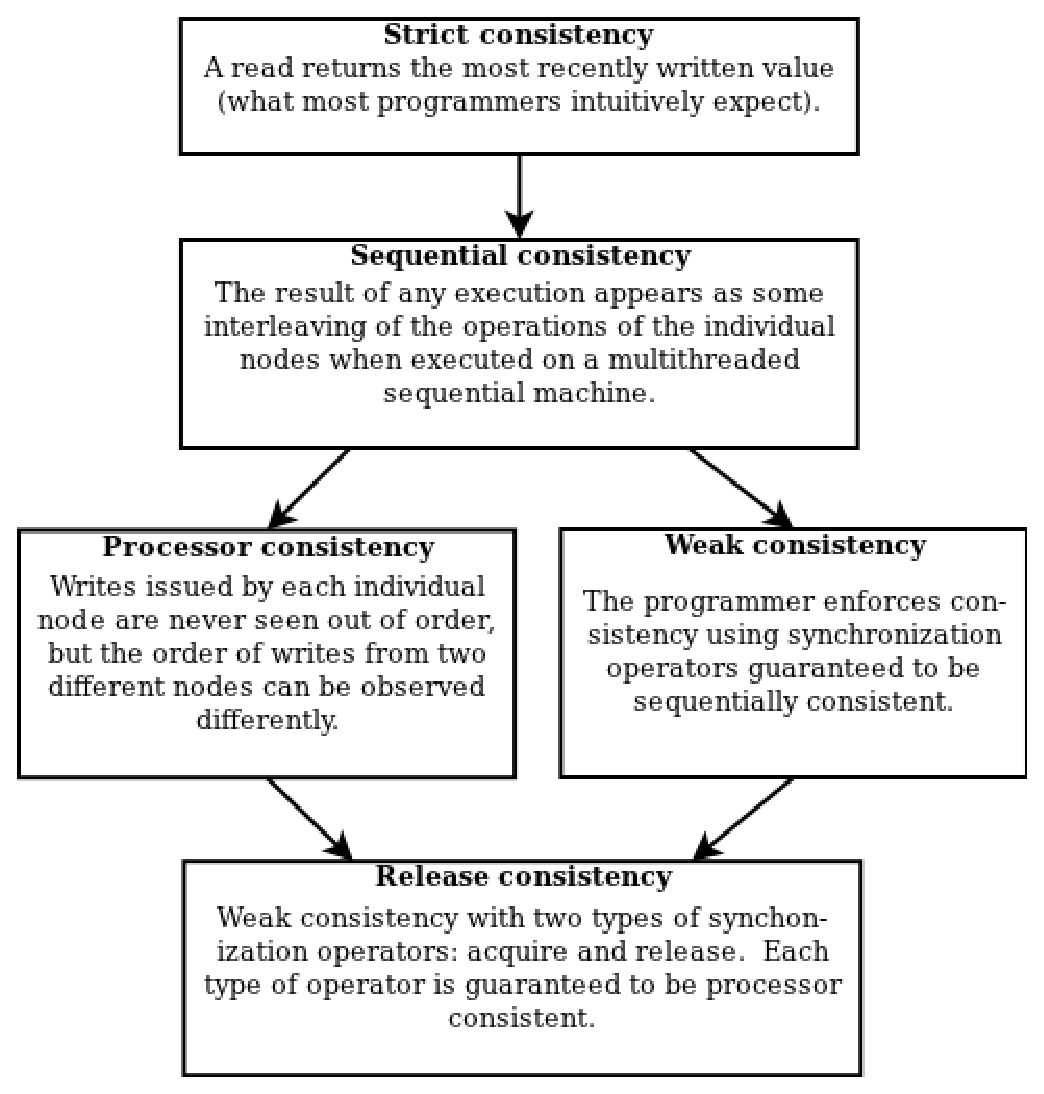
\includegraphics[scale=0.40]{images/memory_consistency.eps}
\caption{Intuitive definitions of memory coherence~\cite{Nitzberg:1991:DSM:112827.112855}.  The arrows point from stricter to weaker consistencies.}
\end{figure}

The remainder of this section depends on the following definitions of a memory access, originally defined by Debois in \cite{Scheurich:1987:CMO:30350.30377, Dubois:1986:MAB:17356.17406} and elaborated on in \cite{Gharachorloo:1990:MCE:325164.325102}.  In the following, $P_x$ refers to a processor $x$.

\begin{quote}
\begin{definition}[Performing a Memory Request]
A $LOAD$ by $P_i$ is considered \em performed with respect to \em $P_k$ at a point in time when the issuing of a $STORE$ to the same address by $P_k$ cannot affect the value returned by the $LOAD$.  A $STORE$ by $P_i$ is considered \em performed with respect to \em $P_k$ at a point in time when an issued $LOAD$ to the same address by $P_k$ returns the value defined by this $STORE$ (or a subsequent $STORE$ to the same location).  An access is \em performed \em when it is performed with respect to all processors.
\end{definition}
\end{quote}
\hfill \\

Additionally, a distinction between \em performed \em and \em globally performed \em $LOAD$ accesses is necessary for architectures with non-atomic $STORE$s.  A $STORE$ is atomic if the value stored becomes readable to all processors at the same time~\cite{Gharachorloo:1990:MCE:325164.325102}.  For DSM systems, it is typically not the case that $STORE$ operations are atomic unless special hardware is used.

\begin{quote}
\begin{definition}[Performing a $LOAD$ Globally]
A $LOAD$ is \em globally performed \em if it is performed \em and \em if the $STORE$ that is the source of the returned value has been performed.
\end{definition}
\end{quote}

\subsection{Strict Consistency}
In order to write programs that correctly execute on a platform, a programmer must understand the memory consistency protocols used on that platform.  The most intuitive protocol programmers expect to see in a platform is \em strict consistency\em~\cite{Goodman:1989:53705}.

As identified by Li and Hudak in \cite{Li:1989:MCS:75104.75105}, a memory is \em coherent \em if the value returned by a read operation is always the value written by the most recent write operation to the same address.  This definition of \em coherent \em memory is exactly what \em strict consistency \em guarantees: a memory read operation returns the most recently written memory value~\cite{Nitzberg:1991:DSM:112827.112855}.  This memory consistency model exhibits the most restrictive rules and serves as a base rule in many of Lamport's formalisms in \cite{Lamport:1979:MMC:1311099.1311750}.  However, because the restrictive rues oftentimes necessitate serial reading and writing, this coherency model is not used in DSM systems whose focus is speed or efficiency.

\subsection{Sequential Consistency}

On platforms with multiple execution paths (e.g., a multi-core processor) programmers expect memory to be \em sequentially consistent\em.  In a \em sequentially consistent \em model, separate processors are expected to be \em strictly coherent\em, but the order of memory access between those processes is defined by the programmer.  A system is sequentially consistent if the result of any execution is the same as if the operations of all the processors were executed in some sequential order, and the operations of each individual process or appear in this sequence in the order specified by its program~\cite{Lamport:1979:MMC:1311099.1311750}.  Dubois studied how one may order events to guarantee sequential consistency in \cite{Scheurich:1987:CMO:30350.30377} by formally demonstrating that ordering $LOAD$ and $STORE$ in a fashion that prevents simultaneous access guarantees correct execution of an application program. 

\subsection{Processor Consistency}

Goodman in \cite{Goodman:1989:53705} introduced the concept of \em processor consistency \em to relax the ordering of \em sequential consistency\em.  Processor consistency requires that memory writes occur strictly consistent only on the executing processor.  To another processor the memory events need not occur in a strictly consistent manner.  Though this consistency model may yield incorrect if the programmer assumes a sequentially consistency, Goodman showed that most applications give the same results because explicit synchronization primitives are used~\cite{Goodman:1989:53705}.  This consistency model is used in combination with weak consistency models to synthesize release consistency models (discussed in Section \ref{release-consistency}).

\subsection{Weak Consistency}
\label{weak-consistency}

When discussing weaker consistency model the discussion is usually limited to two things: correctness and performance.  Correctness is important for showing a weaker consistency model is equivalent to a stricter consistency model in regards to a program's execution.  The main purpose of weaker coherency models is performance~\cite{Gharachorloo:1990:MCE:325164.325102}.  Weaker consistency models can be derived by grouping competing and synchronized memory requests to synchronization points in the program~\cite{Gharachorloo:1990:MCE:325164.325102}.  In practice, this means delaying the ordering of memory events to some synchronization point -- typically, a release or acquire.

This type of coherency protocol provides a sufficient programming environment for programs that require synchronization -- e.g., programs that require serial execution for critical sections and barriers~\cite{Steinke:2004:UTS:1017460.1017464} -- while maintaining a simple programming interface for developer.  Correctness of execution is so because the programmer is expected to coordinate when data may be accessed through synchronization primitives.  More concretely, if a program relies on critical sections to correctly execute, the programmer is responsible for ensuring that the memory written to by the critical sections is not read until all processors are done writing using synchronization primitives provided by the underlying system.

Additionally, it has also been shown in work such as \cite{Scheurich:1987:CMO:30350.30377} and \cite{Scales:1997:TTE:268998.266673} that these weaker consistency models can be implemented invisibility to the application programmer.  By implementing a compiler that invisibly enforces consistency rules, an application written to adhere to a processor consistency memory interface (e.g., written using synchronization primitives to ensure correctness of execution) can be further translated to work on a even weaker memory consistency model.  In the case of Shasta, application programs like Oracle 7.3 database system originally compiled for a single shared-memory multiprocessor were able to successfully run on this release consistent DSM system without any changes to the original application program~\cite{Scales:1997:TTE:268998.266673}.

Gharachorloo provided the following conditions for weak consistency in \cite{Gharachorloo:1990:MCE:325164.325102}:

\begin{quote}
\begin{condition}[Weak Consistency]
(A) before an ordinary $LOAD$ or $STORE$ access is allowed to perform with respect to any other processor, all previous \em synchronization \em accesses must be performed, and (B) before a \em synchronization \em access is allowed to perform with respect to any other processor, all previous ordinary $LOAD$ and $STORE$ accesses must be performed, and (C) \em synchronization \em accesses are sequentially consistent with respect to one another.
\end{condition}
\end{quote}

\subsection{Release Consistency}
\label{release-consistency}

Release consistency is a weak consistency model that further relaxes the restrictions of the consistency model discussed in Section \ref{weak-consistency} by overlapping release and acquire synchronization events.  This additional change differentiates synchronization and regular accesses to memory, which allow release consistent models to exploit access patterns to provide better performance.  This model effectively creates a pipeline of release and acquire events.

\begin{quote}
\begin{condition}[Release Consistency]
(A) before an ordinary $LOAD$ or $STORE$ access is allowed to perform with respect to any other processor, all previous \em acquire \em accesses must be performed, and (B) before a \em release \em access is allowed to perform with respect to any other processor, all previous ordinary $LOAD$ and $STORE$ accesses must be performed, and (C) \em special accesses \em are processor consistent with respect to one another.
\end{condition}
\end{quote}

\subsubsection{Eager \& Lazy Release Consistency}

Several other researchers have formalized the conditions for release consistency in works such as \cite{Gharachorloo:1990:MCE:325164.325102} and \cite{Keleher:1992:LRC:139669.139676}, which serve as a basis for other derived coherency models discussed later in this section:

The two main variants of release consistency in literature are \em eager release consistency \em and \em lazy release consistency\em.  These two coherency models are used by the major of software DSM systems, such as Treadmarks in \cite{Amza:1996:TSM:226705.226708,Keleher:1994:TDS:1267074.1267084}, Munin in \cite{Keleher:1992:LRC:139669.139676, Bennett:1990:MDS:99163.99182, Carter:1991:IPM:121132.121159, Zwaenepoel:1992:MDS:134397.135235} and Shasta in \cite{Scales:1996:SLO:237090.237179}.  Each of these derivatives obey the conditions for release consistency derived in \cite{Gharachorloo:1990:MCE:325164.325102}, but treat communication differently.  As the names suggest, \em eager release consistency \em communicate memory accesses as they happen, whereas \em lazy release consistency \em delays communication of memory accesses until some prescribed event occurs.

\paragraph{Eager Release Consistency (ERC)} ERC protocols delay propagating its modifications to shared data until a \em release \em synchronization access and is studied in \cite{Keleher:1992:LRC:139669.139676}.  At the time of a \em release\em, the ERC protocol propagates modifications to all other processors that cache the memory page.  A naive implementation of an ERC protocol may propagate these changes at the \em release \em or send invalidate requests to processors working on the memory page.  However, regardless of the implementation details of the ERC protocol, significant overhead is incurred by communicating changes at each \em release \em event.

\paragraph{Lazy Release Consistency (LRC)} LRC protocols delay propagating its modifications to shared data until an \em acquire \em synchronization access and is studied in \cite{Keleher:1992:LRC:139669.139676}.  At the time of an \em acquire\em, the LRC protocol propagates modifications to the requesting processor by piggybacking the changes to the memory page on a successful \em acquire \em message~\cite{Keleher:1992:LRC:139669.139676}.  Optimizations also exist that can allow an acquiring processor to only request changes that it actually needs.

\section{System Design}
\label{system-design}

The \projname{} system presented in this paper is a software distributed shared memory systems.  Like Treadmarks in \cite{Amza:1996:TSM:226705.226708,Keleher:1994:TDS:1267074.1267084}, the \projname{} system is implemented entirely in user-space, making complicated kernel-based modifications unnecessary.  The \projname{} system features a centralized manager and is designed to use the respective servers presented by Li and Hudak in \cite{Li:1989:MCS:75104.75105}.  The \projname{} system maintains an unstructured memory region.  In fact, it makes no modifications to the memory structure used by the underlying application unless otherwise noted.  This allows the \projname{} system to be used by any application without the need for source code modification, as is the case in some type-specific coherence systems that may require annotations to label memory.  Research has shown that lazy release consistency is an ideal memory coherence model for SDSM systems.  As such, the \projname{} system will be designed to exhibit a lazy release memory coherence model.  For comparison, the \projname{} system will be able to exhibit other memory coherence models, too, depending on what application synchronization primitives are used.

This chapter discusses the assumptions, design considerations, and design decisions of the \projname{} system.  The implementation of the design presented in this chapter is the subject of future chapters.

\subsection{Assumptions}
\label{assumptions}

There are several assumptions that were necessary to make for implementation reasons.  The following is a discussion of each of those assumptions, as well as a brief discussion regarding why the assumption was necessary.

\begin{description}
\item[Operating System] \hfill \\
The \projname{} system requires that the distributed system be run on identical operating systems.  This is partly due to the system's reliance on the application binary (e.g., exported symbols) and program loader (e.g., placement of loadable segments).  This assumption assumes that the same compilation toolchain is used on each member of the cluser.

\item[Threading Library Requirements] \hfill \\
 The \projname{} system is designed to distribute work across multiple execution cores.  The only feasible way to do this is to require that the target application be written using a threading library.  The \projname{} system requires that the target application use the \verb,pthread, library, and also assumes that the target application is properly written using appropriate \verb,pthread, provided synchronization primitives like \verb,pthread_mutex,.  Currently, the \projname{} system only supports \verb,pthread_mutex,.

\item[Compilation Requirements] \hfill \\
The \projname{} system is a shared library.  As such, the target application must be linked with and loaded with the \projname{} library.  This allows \projname{} to replace function definitions for important functions like \verb,pthread_create, and \verb,malloc,.
\end{description}


\subsection{Virtual Memory Management Design}
\label{vmm-design}

Typical virtual memory management (VMM) systems operate in kernel-space, hiding virtually all aspects of memory management to the application programmer.  For many types of applications this is permissible, and even preferred.  However, for a SDSM system built in user-space, the transparent management of memory is a problem that must be addressed by emulating its behavior in user-space.

Running a VMM in user-space is non-trivial and requires understanding and control of many system-specific phenomena.  The understanding and control required is compounded when more than one process running separate address spaces are expected to use the same VMM.  These challenges and system-specific phenomena are the topic of this section.

\subsubsection{Address Space Utilization}
Virtual memory fools application programs to believe the program has access to a contiguous range of memory.  The system provided VMM does this by mapping process identification and virtual addresses to available physical addresses located in physical memory via lookup tables like the \em page table\em.  This is done transparently.  That is, an application never sees or requires the address of a physical page of memory.  Rather, these tasks are that of the underlying kernel.  For applications that wish to manage memory themselves or for other applications, this is problematic because the underlying placement of memory is invisible to the application.  This makes synchronizing memory between multiple processes challenging.

The strategy taken the \projname{} system is to leave the system provided VMM in place and add an additional user-space VMM to the application program.  This has the advantage of allowing one to record the placement of virtual pages, while leaving the task of mapping the virtual page into the underlying system's physical memory.  The truth is, for a SDSM system one does not care what physical memory is being used.

Using this design, the \projname{} system can broadcast what memory it has available in each of the nodes' virtual memory without the need to know about each nodes' underlying physical memory.  It is the task of the user-space VMM to then synchronize available memory and memory permissions to participating nodes.

\subsubsection{Address Space Synchronization}

We have assumed that the \projname{} system is compiled as a shared library, and that the target application is linked and loaded with this shared library.  As a result, the library code exists in the same address space as the target application during the lifetime of the application.  This has several non-obvious implications that make building a distributed VMM difficult.  

A naive VMM design places \projname{} heap allocated memory in the target application's heap area.  This has the effect of mixing \projname{} heap allocated memory with the target application's heap allocated memory.  The problem of deciphering what memory is belongs to \projname{} versus what memory is belongs to the target application is difficult.  This problem is compounded when one considers that \projname{}'s and the target application's heap allocated memory are mixed on a single memory unit.  Additionally, heap addresses tend to differ between processes which necessitate tedious memory remapping.  This makes synchronization virtually impossible.

Therefore, the first challenge is that of enforcing a clean separation of \projname{} heap allocated memory from the target application's heap allocated memory.  By enforcing a clean separation of \projname{} from the target application, the problem of synchronization is far less difficult.  Using this design, \projname{} may maintain a VMM in a separate region of memory that can be synchronized with other \projname{} instances in the cluster.  Additionally, this allows us to fix critical \projname{} memory addresses in memory.  Because we have assumed we're running the same target application on the same underlying architecture, we can use fixed addresses and offsets to choose a safe area for \projname{}'s heap.  Lastly, because an entire region of memory is being synchronized between projects, objects like those in the Standard Template Library can be used between processes.  This makes building complex data structures simple.

\subsubsection{Fault Resolution}

A distributed node, having been alerted to the shared memory mappings of the network cluster, needs a mechanism to access the memory that may not be mapped into its own virtual memory.  Functionally, this allows a distributed node to read and write memory that another distributed node has mapped into its own virtual memory address space.

To achieve this, Linux signal handling tools may be employed to detect and resolve memory access attempts.  For example, one may detect memory accesses by using the \verb,mprotect, system call to set access permissions on memory pages.  Furthermore, illegal accesses to these memory pages will result in the generation of a \verb,SIGSEGV, signal.  By designing a signal handler for \verb,SIGSEGV, one may enforce permissions on memory.  Additionally, one may even resolve the illegal memory access by remapping memory and allowing the offending instruction to \em try \em access memory again.  Ideally, after remapping memory, the offending instruction will execute without illegally accessing memory.  This strategy is identical to the strategy used by Treadmarks in \cite{Keleher:1994:TDS:1267074.1267084}.

\subsection{Network Cluster Coordinator}
\label{network-stack-design}

\subsubsection{Bootstrapping}
Bootstrapping a distributed shared memory system is a non-trivial task that requires careful handling of several items closely related to the underlying system.  The most important tasks include the loading of the target-application and verification and comparison of address spaces features.  Loading an application designed to run on a single machine is a trivial problem where most system-specific intricacies are hidden from the application programmer by their system-provided toolchain.  However, loading an application designed to run on a single machine on a cluster of machines is non-trivial.

Because of the assumptions that the \projname{} system maintains in regards to compilation requirements and operating system similiarity, we designed \projname{} in a fashion that allows us to run a \em single \em application binary on each networked machine.  This \em single \em application binary contains all code to operate as both a master and a worker.  This application binary is compiled, linked and loaded with the same compiler toolchain and and loaded on identical architectures.  This has several beneficial side-effects.  Firstly, a single application is distributed between the nodes.  Secondly, the object file on disk is identical.  Because the same toolchain and operating systems is required, the loaded process image guarantees address space uniformity: loadable segments share the same addresses.  The only items that aren't guaranteed to be identical is the dynamic linker's placement choices for shared libraries.  However, in practice we've seen that they are similiar enough.  We use heuristics to identify where process-specific shared libraries exist and take measures to ensure that each process is aware of the placement of other processes' shared libraries.

Another non-obvious challenge that the bootstrapping design must address is a facility to hault the target-application until a message or signal is passed to it.  Applications designed to run on a single machine need not worry about this design issue because once an application is loaded it is ready to run code -- presumably its \verb,main, entrypoint.  This is not the case in a distributed system.  The \projname{} bootstrapping system is tasked with determining a master node, waiting for worker nodes to join and initialize themselves, and lastly, signalling a \em single \em target-application to call its entry point.

\subsubsection{Cluster Coordination}
There are several networking facilities that the \projname{} system must be able to support.  These facilities are a combination of multicast and unicast communication styles.  However, the ability to communicate with other nodes is a trivial problem.  Instead, the task of the cluster coordinator is really to detect \em when \em certain networking events should happen.  For example, \em when \em should a master node synchronize its data with a new worker or \em when \em should a master create or join threads on a worker node are events that the cluster coordinator must identify.

Because of the assumption that the target-application is a \verb,pthread, based program linked with the \projname{} library, we can make use of several system tricks to help identify interesting events.  First, the \projname{} library can make use of symbol manipulation to replace the implementations of functions like \verb,pthread_create, or \verb,pthread_join, with different implementations with stronger linkage.  Second, the \projname{} system can make use of allocator hooks to instrument or completely replace the implementation of \verb,malloc, and \verb,free,.  Combining these strategies provides a solid foundation to populate an event queue capable of powering a SDSM system.

The \projname{} system requires an event-driven networking infrastructure to communicate the events previously described.  We found that using a mixture of multicast and unicast datagrams made the implementation most straight-forward.  Furthermore, we found that using a single client-server combination was inappropriate, and opted to maintain multiple servers per-process.  Among other reasons, using this design the \projname{} system is capable of performing blocking work without halting the servers responsible for listening and queueing important events in the cluster.


\subsubsection{Coherence Semantics}
One of the most important features the \projname{} system must support is a weak memory coherency model.  Though a DSM system may operate correctly using a stricter coherency model, efficiency and communication overhead become serious concerns.  Supporting a weak coherency model maximizes efficiency by minimizing the communication overhead involved in maintaining a global address space.

To implement such a coherency model, the \projname{} system needs to know certain information about the access patterns the target-application exhibits.  In systems like Munin~\cite{Keleher:1992:LRC:139669.139676, Bennett:1990:MDS:99163.99182, Carter:1991:IPM:121132.121159, Zwaenepoel:1992:MDS:134397.135235}, this is done through memory annotations.  This model was considered too restrictive for \projname{}, as it requires source code annotations or an intelligent runtime system to categorize memory accesses.  Because of the assumption that the target-application is a \verb,pthread, based program, we can exploit synchronization primitives like \verb,pthread_mutex,s to enforce a weaker consistency model.  

A weak consistency model can be designed in \projname{} by intercepting \verb,pthread_mutex_lock, and \verb,pthread_mutex_unlock,.  When a worker node acquires a lock and receives confirmation that the lock was acquired from the central manager, that worker can record what pages are dirtied during its execution.  Upon releasing the lock, that worker can transmit what pages it has invalidated to the central manager.  The central manager can then lazily propagate these invalidated pages to future acquirers of the same mutex.  This approach hangs program correctness on the locking used in the application.

This approach requires no \em additional \em source code annotations.  We feel that assuming correctly written applications is a reasonable assumption.  There are several interesting caveats that must be taken into consideration when determining what types of applications are correctly written.  For example, most \verb,pthread, based applications can make the assumption that the threads are running within the same address space on the same machine.  This assumption often leads to a program that allows threads to read or write memory concurrently without the use of locks or barriers, as long as those threads are not reading and writing the \em same \em memory concurrently.  One practical example of this type of application is a \verb,pthread,-enabled version of matrix multiply.  Running this type of application on a DSM will be inefficient because of the potential for the threads to thrash over the ownership of a memory page.  Applications that do not make this assumption and use locks and barriers to synchronize read and write accesses to memory will realize the full power of the weaker consistency models.





\section{System Implementation}

\subsection{Overview}
Talk about process structure and define all of our vocabulary we're using in this chapter.

\subsection{Virtual Memory Management}
\subsubsection{Page Table}
Talk about \verb,node_list, and \verb,page_table,.  Talk about how we can cast it as a \verb,std::map, and why we use placement new (mention shared libraries being loaded into random addresses, so we needed a fixed place to put all this stuff).

\subsubsection{Fault Handling}

\subsection{Cluster Coordinator}

\subsubsection{Bootstrapping}
Talk about the auto-configuring cluster.  Talk about how we verified address spaces.  Talk about sync'ing the page table.

\subsubsection{Communication}
\subsubsection{Coherence Protocol}

\subsection{Threading}
Talk about \verb,pthread, code that we replaced and why.
\section{Results}

In this section we show how long it takes to resolve a fault over the network and we compare \projname{} to \verb,malloc, in several tests.

\subsection{Fault duration}


\subsection{Malloc vs. \projname{}}

The program used to test was a matrix multiplcation program from Stanford.

\subsubsection{Fixed matrix size, varying number of threads}

In this test we kept the matrix size fixed at 200x200 and we varied the number of worker threads betweem 1 and 4.

\begin{figure}[!h]
\centering
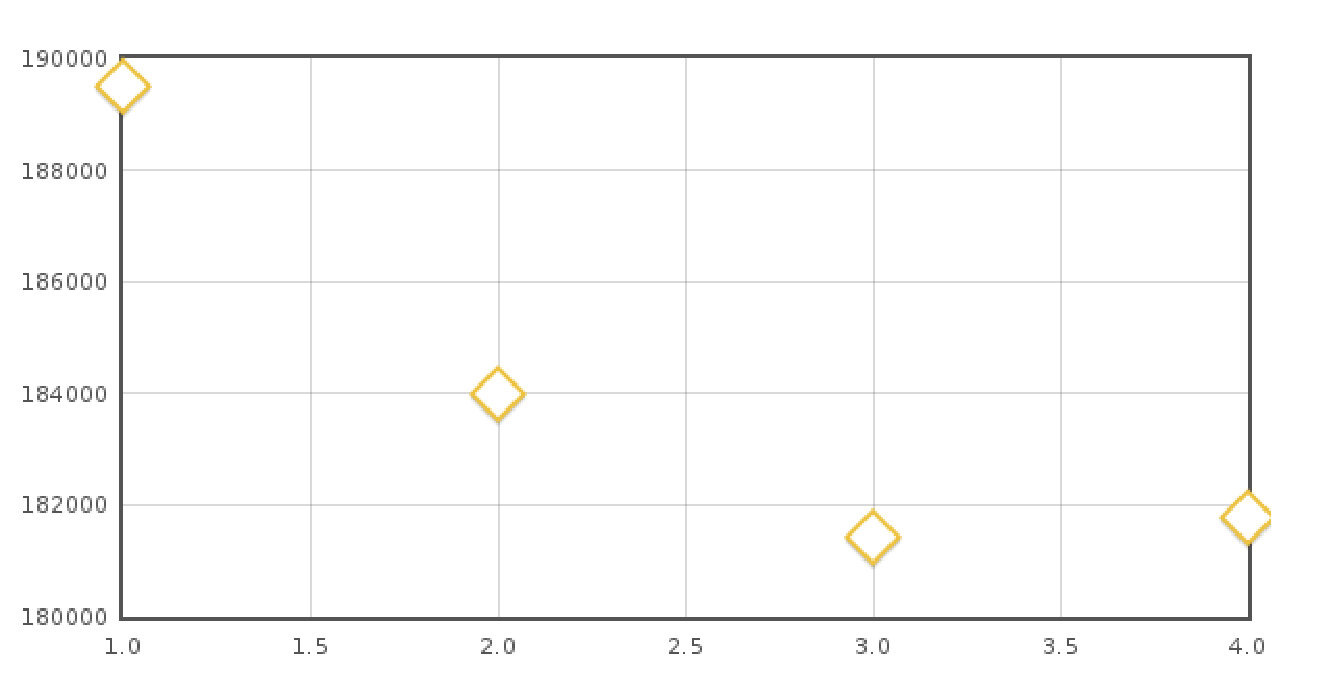
\includegraphics[scale=0.40]{images/malloc-fixed-matrix.eps}
\caption{Malloc: The x axis the number of threads used. The y axis is time to run the test in microseconds.}
\end{figure}

\begin{figure}[!h]
\centering
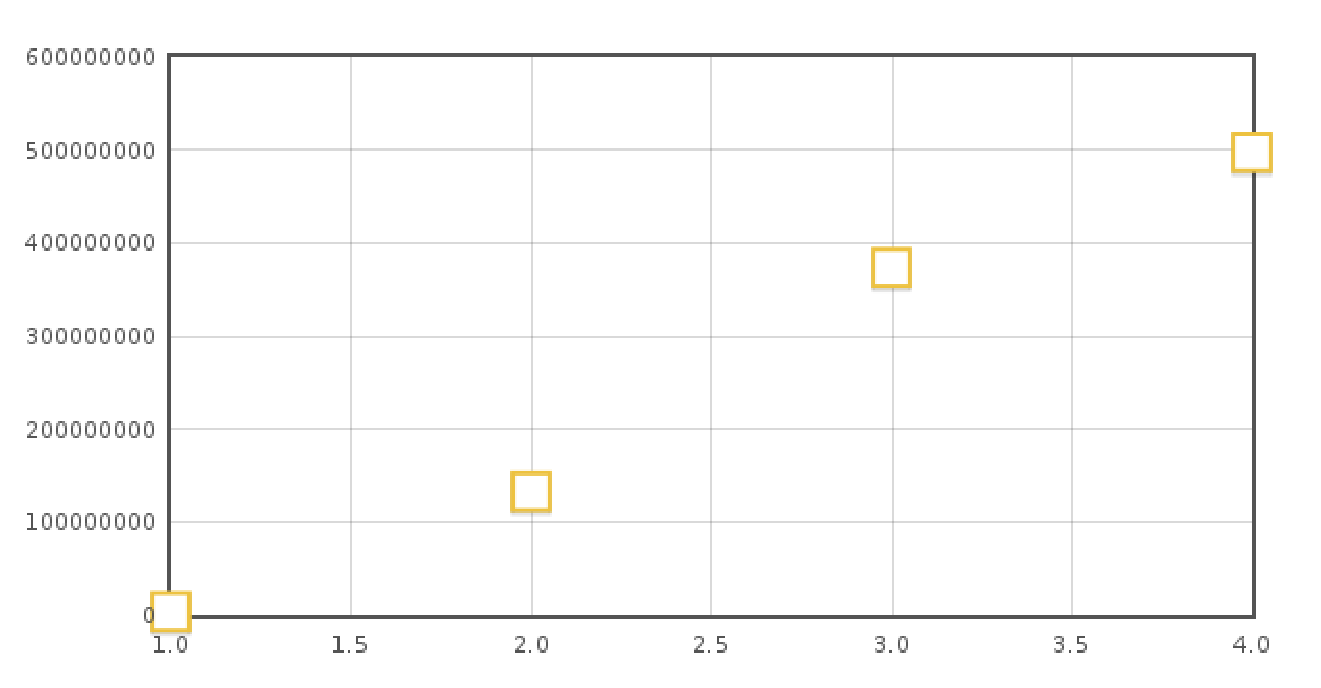
\includegraphics[scale=0.40]{images/mmult-lh-fixed-size.eps}
\caption{\projname{} with processor consistency: The x axis the number of threads used. The y axis is time to run the test in microseconds.}
\end{figure}

\begin{figure}[!h]
\centering
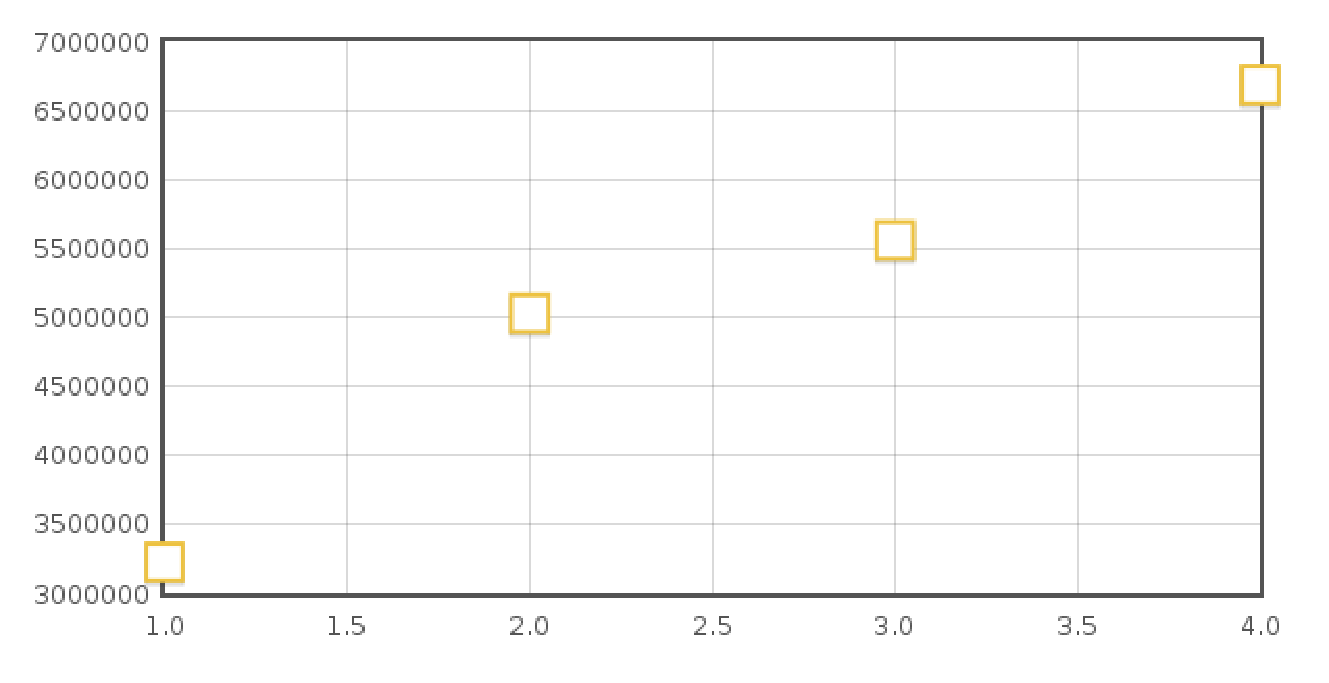
\includegraphics[scale=0.40]{images/mmlh-fixed-size.eps}
\caption{\projname{} with release consistency: The x axis is matrix size. For example, 100 refers to multiplying 2 100x100 matrixes. The y axis is time to run the test in microseconds.}
\end{figure}

\verb,Malloc, vastly outperforms \projname{} with processor consistency no matter how many threads are used.  This has to do with not having read-only pages.  Every time a worker needs to do work it invalidates all other workers copies of that page.  This ends up with the workers thrashing over pages.  It was expected when we began this test that \projname{} with processor consistency would yield worse results as the number of threads increased because of the trashing issues.

With release consistency, \projname{} achieves much better performance than processor consistency.  For 4 threads, release consistency only takes around 66 seconds.  Compared to processor consistency taking around 500 seconds.  Release consistency still loses to the \verb,malloc, version.  One reason why is because the workers end up thrashing over the write pages.

\subsubsection{Fixed thread count, varying matrix size}

In this test we kept the number of worker threads fixed at 4 and we varied the matrix size.

\begin{figure}[!h]
\centering
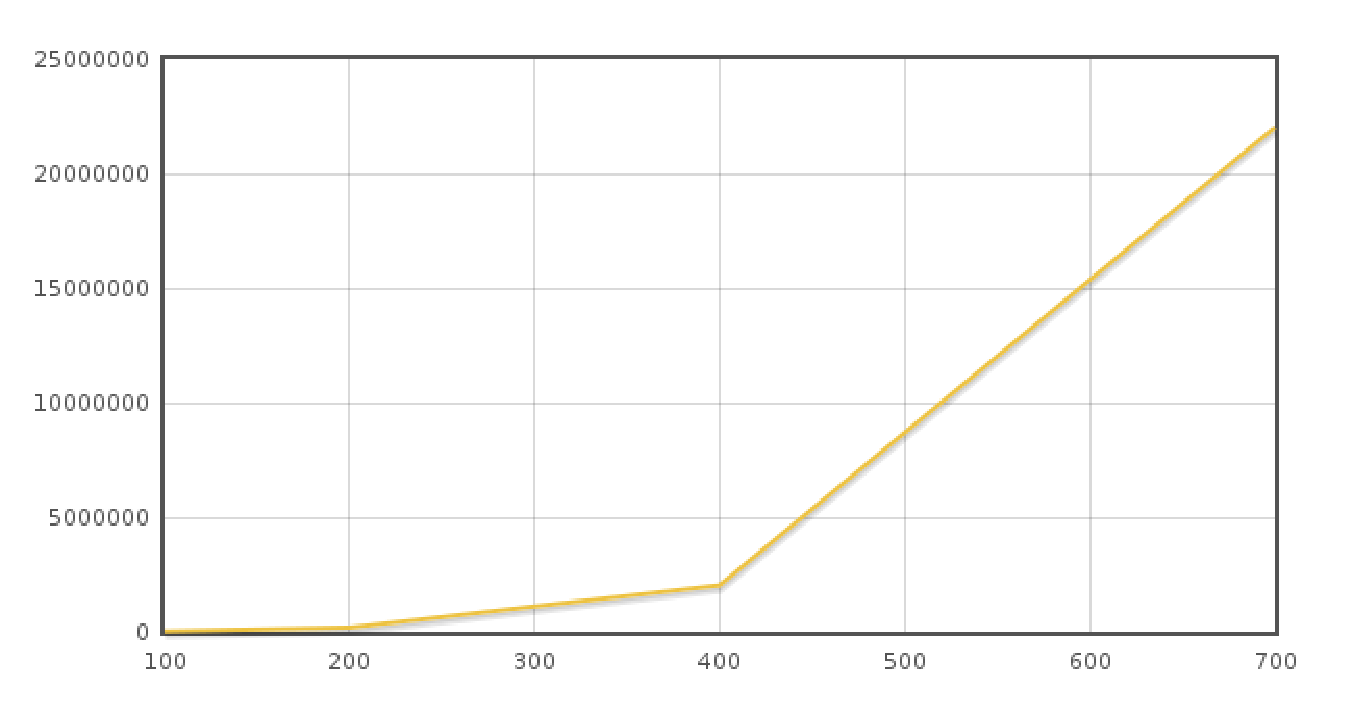
\includegraphics[scale=0.40]{images/malloc-fixed-thread.eps}
\caption{Malloc: The x axis is matrix size. For example, 100 refers to multiplying 2 100x100 matrixes. The y axis is time to run the test in microseconds.}
\end{figure}

\begin{figure}[!h]
\centering
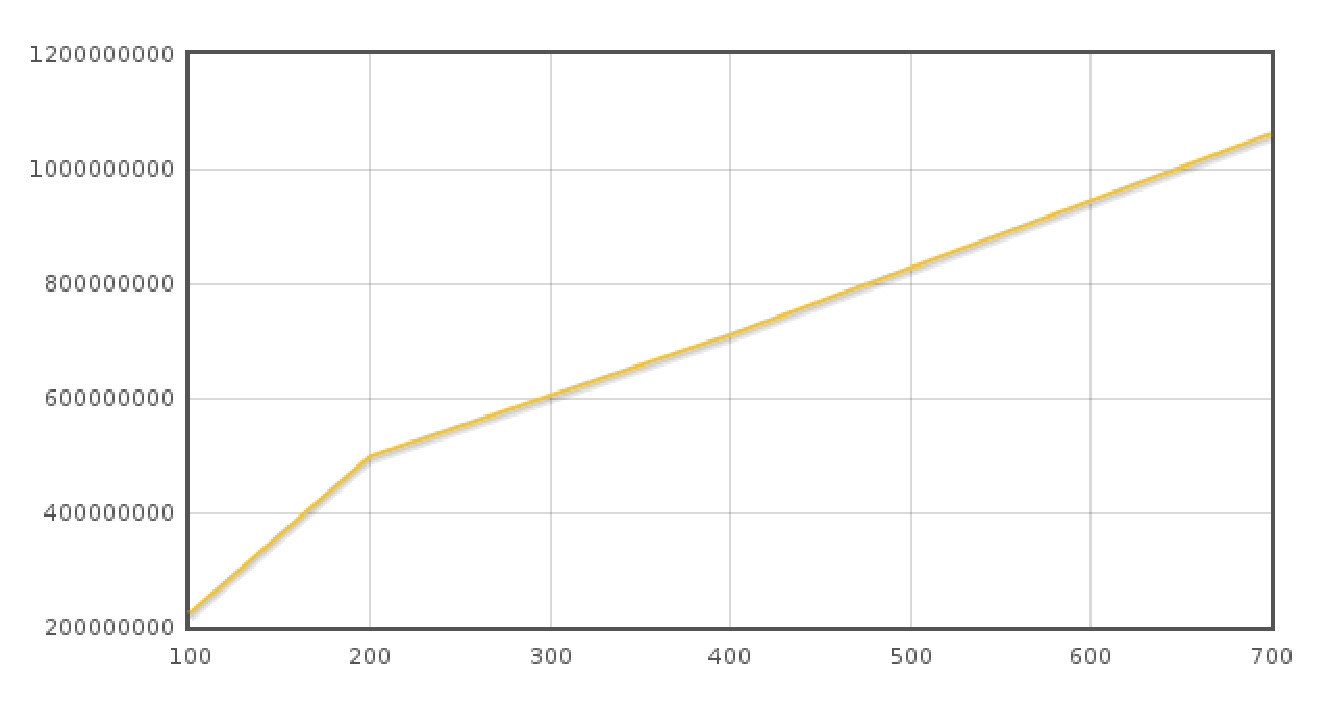
\includegraphics[scale=0.40]{images/mmult-lh-fixed-thread.eps}
\caption{\projname{} with processor consistency: The x axis is matrix size. For example, 100 refers to multiplying 2 100x100 matrixes. The y axis is time to run the test in microseconds.}
\end{figure}

\begin{figure}[!h]
\centering
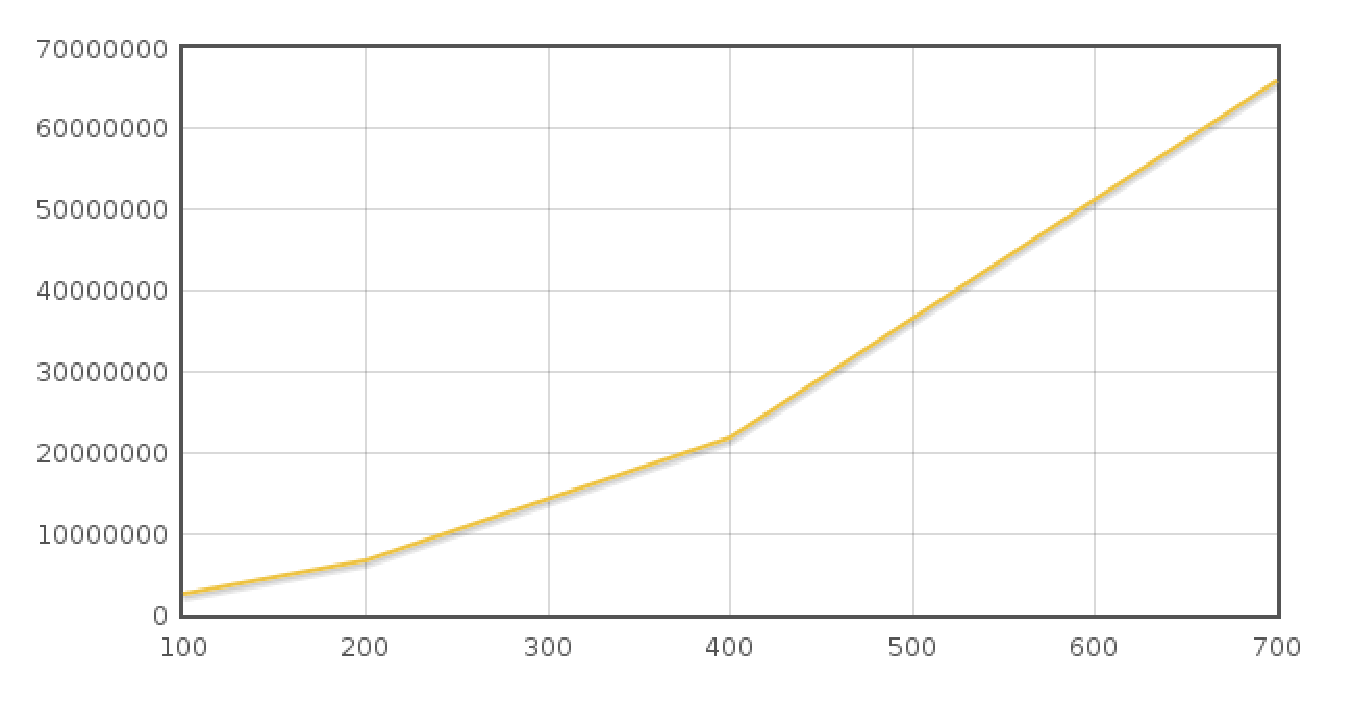
\includegraphics[scale=0.40]{images/mmlh-fixed-threads.eps}
\caption{\projname{} with release consistency: The x axis is matrix size. For example, 100 refers to multiplying 2 100x100 matrixes. The y axis is time to run the test in microseconds.}
\end{figure}

Again, like in the previous test \verb,malloc, vastly outperforms \projname{} with processor consistency at any matrix size. \projname{} with processor consistency gets hit hard by not having read only pages. It ends up transferring the 2 matrixes being multiplied a ton thereby having a horrific runtime.

With release consistency, \projname{} achieves much better performance than processor consistency. Again, release consistency still loses to the \verb,malloc, version because the workers end up thrashing over the write pages. It is still impressive that the release consistency version multiplying a 700x700 matrix finishes in around 66 seconds. The processor consistency version of the project was destroyed by that test and ended up taking over 1000 seconds.



\bibliographystyle{IEEEannot}
\bibliography{nlcbsmm}
\end{document}
